\chapter[Modal Example II: Other Methods]{Modal Example II\\Other Methods}

For comparison, other solution methods are applied to the Bevington data. These methods will reinforce the geometry of least squares.

\section{\label{sec:normal II}Normal Equations from Vectors}  %    S    S    S    S    S    S    S    S    S
In \S \ref{sec:normal I}, the normal equations appeared from the linear system resulting from the two partial differential equations in \eqref{eq:bev pde}. Another approach starts with the linear equation $\axeb$ and uses column vectors. The data is posed in terms of the column vectors in table \ref{tab:bevington data and results}. These, plus a constant vector, are the elements of composition:
  \begin{equation*}   %  =   =   =   =   =
    {\bf{1}} = \mat{c}{1 \\ 1 \\ 1 \\ 1 \\ 1 \\ 1 \\ 1 \\ 1 \\ 1}, \quad
    x        = \mat{c}{1 \\ 2 \\ 3 \\ 4 \\ 5 \\ 6 \\ 7 \\ 8 \\ 9}, \quad
    T        = \frac{1}{10} \mat{c}{156 \\ 175 \\ 366 \\ 438 \\ 582 \\ 616 \\ 642 \\ 704 \\ 988}.
    %\label{eq:}
  \end{equation*}
There are two column vectors in the system matrix $\A{}$:
  \begin{equation*}   %  =   =   =   =   =
    \A{} = 
      \mat{c|c}{{\bf{1}} & x}
    %\label{eq:}
  \end{equation*}
In the service of a crisp mental image, the linear system is written explicitly:
  \begin{equation}   %  =   =   =   =   =
  \begin{array}{cccc}
      \A{} & a & = & T \\
      \mat{cc}{
         1 & 1 \\
         1 & 2 \\
         1 & 3 \\
         1 & 4 \\
         1 & 5 \\
         1 & 6 \\
         1 & 7 \\
         1 & 8 \\
         1 & 9 } &
      \mat{c}{ a_{0} \\ a_{1} } & = &
         \frac{1}{10} \mat{c}{156 \\ 175 \\ 366 \\ 438 \\ 582 \\ 616 \\ 642 \\ 704 \\ 988} .
    \label{eq:bevington axeb}
  \end{array}
  \end{equation}

\subsection{Composing the normal equations}  %   SS   SS   SS   SS   SS   SS   SS   SS   SS   SS   SS   SS
The system encodes nine linear problems:
  \begin{equation*}   %  =   =   =   =   =
   \begin{split}
    a_{0} + a_{1} x_{1} & = T_{1}, \\
     & \ \, \vdots \\
    a_{0} + a_{1} x_{9} & = T_{9}.
    %\label{eq:}
    \end{split}
  \end{equation*}
But there are no parameters $a_{0}$ and $a_{1}$ which solve all nine equations. More formally, the data vector $T$ is not in the column space of $\A{}$. There are no parameters $a_{0}$ and $a_{1}$ such that
  \begin{equation*}   %  =   =   =   =   =
    a_{0} {\bf{1}} + a_{1} x = T.
  \end{equation*}
One strategy is to compose a solution does have a solution
  \begin{equation*}   %  =   =   =   =   =
    \wx{*} a = \A{*} T.
  \end{equation*}
Certainly the vector $\A{*} T$ is in the column space of $\A{*}$ -- the coordinates are $T$! The solution is
  \begin{equation*}   %  =   =   =   =   =
    \mat{c}{a_{0} \\ a_{1}} = \wxi{*} \A{*}T.
  \end{equation*}
For the Bevington data set the dot products are,
  \begin{equation*}   %  =   =   =   =   =
  \begin{split}
    \oto &= m = 9, \\
    \otx &= \xto = 45, \\
    \xtx &= 285, \\
    {\bf{1}}^{\mathrm{T}}T &= \frac{4667}{10}, \\
    x^{\mathrm{T}}T        &= 2898.
    %\label{eq:}
  \end{split}
  \end{equation*}
Other intermediate products include the product matrix,
  \begin{equation*}   %  =   =   =   =   =  
     \wx{*} = \mat{cc}{\oto & \otx \\ \xto & \xtx} = \mat{cc}{9 & 45 \\ 45 & 285},
  \end{equation*}
its determinant,
  \begin{equation}   %  =   =   =   =   =
    \Delta = \paren{\oto} \paren{\xtx} - \paren{\otx}^{2},
    \label{eq:det again}
  %\end{split}
  \end{equation}
inverse,
  \begin{equation*}   %  =   =   =   =   =
  %\begin{split}
    \wxi{*} = \Delta^{-1} 
      \mat{rr}{\xtx & -\oto \\ -\oto & \otx}
    %\label{eq:}
  %\end{split}
  \end{equation*}
and the vector,
  \begin{equation*}   %  =   =   =   =   =
    \A{*}T = 
      \mat{c}{{ \bf{1}}^{\mathrm{T}}T \\ x^{\mathrm{T}}T } =
      \frac{1}{10} \mat{c}{4667 \\28\,980}.
  \end{equation*}
The solution is again
  \begin{equation*}   %  =   =   =   =   =
  %\begin{split}
    a = \Delta^{-1} 
      \mat{rr}{\xtx & -\oto \\ -\oto & \otx} 
      \mat{c}{{ \bf{1}}^{\mathrm{T}}T \\ x^{\mathrm{T}}T }
    %\label{eq:}
  %\end{split}
  \end{equation*}
  \begin{equation}   %  =   =   =   =   =
  %\begin{split}
    \mat{c} {a_{0} \\ a_{1}} = \Delta^{-1}
    \mat{c}{ \paren{\xtx} \paren{\mathbf{1}^{\mathrm{T}}T} -
             \paren{\otx} \paren{x^{\mathrm{T}}T} \\
             \paren{\oto} \paren{x^{\mathrm{T}}T} -
             \paren{\otx} \paren{\mathbf{1}^{\mathrm{T}}T} }
    \label{eq:bevington:soln:vectors}
  %\end{split}
  \end{equation}
leading to the same solution presented in \S \ref{sec:exact form}.

\section{Singular Value Decomposition}  %    S    S    S    S    S    S    S    S    S
The \asvd \ is an $x-$ray revealing the structure of the fundamental spaces.

\subsection{Computing the SVD}  %   SS   SS   SS   SS   SS   SS   SS   SS   SS   SS   SS   SS
Solution steps
\begin{enumerate}
  \item Compute $\lambda\paren{\wx{*}}$.
  \item Educated guess at domain matrix $\V{}$.
  \item Compute codomain matrix $\U{}$.
\end{enumerate}
The least squares problem delivers a singular value decomposition (SVD) without the muss and fuss of solving an eigensystem. The SVD is given by the matrix product
  % = =  e q u a t i o n
  \begin{equation*}
    \aesvd{*}.
  \end{equation*}
  % = =
For the full column rank problem we have we can expand in the following block decomposition
  % = =  e q u a t i o n
  \begin{equation*}
    \A{} = \csvdblockbc{*}
  \end{equation*}
  % = =
The $\ess{}$ matrix contains the singular values
  % = =  e q u a t i o n
  \begin{equation*}
    \ess{} = \mat{cc}{\sigma_{1} & 0 \\ 0 & \sigma_{2}}.
    %\label{eqn:}
  \end{equation*}
  % = =
The column vectors of the matrix $\bvr{}$ represent an orthonormal basis for the row space (domain). The column vectors of the matrix $\bur{}$ represent two of the nine vectors in an orthonormal basis for the column space (codomain).

\subsubsection{Singular values}  %  SSS  SSS  SSS  SSS  SSS  SSS  SSS  SSS  SSS  SSS  SSS  SSS
The singular value spectrum of the matrix $\A{}$ is the square root of the (non-zero) eigenvalues of the product matrix $\wx{*}$
  % = =  e q u a t i o n
  \begin{equation*}
    \sigma \paren{\A{}} = \sqrt{\lambda\paren{\wx{*}}}.
    %\label{eqn:}
  \end{equation*}
  % = =
The eigenvalues of the product matrix are the roots of the characteristic polynomial $p(\lambda)$ for said matrix.
  % = =  e q u a t i o n
  \begin{equation*}
    p(\lambda) = \lambda^{2} - \lambda \, \tr{\wx{*}} + \det\paren{\wx{*}}
    %\label{eqn:}
  \end{equation*}
  % = = 
The determinant appeared in equations \eqref{eq:det} and \eqref{eq:det again}; the trace is  $\tr{\wx{*}}=\oto+\xtx$. The singular values are then
  % = =  e q u a t i o n
  \begin{equation*}
    \sigma = \sqrt{\half \paren{\oto+\xtx \pm \sqrt{4\paren{\otx}^{2} - \paren{\oto-\xtx}^{2}}}} .
  \end{equation*}
  % = =
(The astute reader will notice that the discriminant does not seem to have the familiar form of $b^{2}-4ac$. The earnest reader will discover why this is so.)
The singular value spectrum for these data is
  % = =  e q u a t i o n
  \begin{equation*}
    \sigma = \sqrt{3\paren{49 \pm \sqrt{2341}}}
    \approx \paren{17.0924, 1.35954} .
    %\label{eqn:}
  \end{equation*}
  % = =
We now have the sigma matrix and the matrix of singular values $\ess{}$:
% = =  e q u a t i o n
  \begin{equation*}
        \sig{} = \mat{c}{\ess{}\\\hline\zero} = \mat{cc}{\sigma_{1} & 0 \\ 0 & \sigma_{2} \\\hline 0 & 0 \\ 0 & 0 \\ 0 & 0 \\ 0 & 0 \\ 0 & 0 \\ 0 & 0 \\ 0 & 0} \approx \mat{cc}{17.0924 & 0 \\ 0 & 1.35954 \\\hline 0 & 0 \\ 0 & 0 \\ 0 & 0 \\ 0 & 0 \\ 0 & 0 \\ 0 & 0 \\ 0 & 0}.
      %\label{eqn:}
  \end{equation*}
% = =

\subsubsection{Domain matrix}  %  SSS  SSS  SSS  SSS  SSS  SSS  SSS  SSS  SSS  SSS  SSS  SSS
We can skip the eigenvector problem. To find the domain matrix we exploit the \asvd \ of the product matrix
% = =  e q u a t i o n
  \begin{equation*}
        \sig{T} \sig{} = \mat{cc}{\ess{}&\zero}\mat{c}{\ess{}\\\zero} = \ess{2}
      %\label{eqn:}
  \end{equation*}
% = =
  % = =  e q u a t i o n
  \begin{equation}
    \bvr{} \ess{2} \bvr{*} = \wx{*} .
    \label{eq:decompwx}
  \end{equation}
  % = =
By the singular value theorem the matrix is unitary and will be a rotation matrix, a reflection matrix or a convolution. We begin by trying a rotation matrix
  % = =  e q u a t i o n
  \begin{equation}
    \bvr{} = \brot{\theta}
    \label{eq:vrot}
  \end{equation}
  % = =
which is colored blue because the column vectors belong to $\brnga{*}$. 
The objective is to find the angle $\theta$. The immediate result of equations \eqref{eq:wxthatmat}, \eqref{eq:decompwx}, and \eqref{eq:vrot} is 
  % = =  e q u a t i o n
  \begin{equation*}
    \begin{split}
      \brot{\theta} \ess{2} \brot{\theta}^{\mathrm{T}} &= \wx{*}, \\[5pt]
      \mat{cc}{\sigma_{1}^{2}\costs + \sigma_{2}^{2}\sints & \paren{\sigma_{1}^{2} - \sigma_{2}^{2}}\cst \\[3pt]
             \paren{\sigma_{1}^{2} - \sigma_{2}^{2}}\cst & \sigma_{2}^{2}\costs + \sigma_{1}^{2}\sints } &=
    \thatmat{} .
    \end{split}
  \end{equation*}
  % = =
which presents multiple solution paths for the angle $\theta$. For example
  % = =  e q u a t i o n
  \begin{equation}
    \cost = \sqrt{\frac{\sigma_{2}^{2} - \oto}{\sigma_{2}^{2} - \sigma_{1}^{2}}} = \sqrt{\frac{\xtx - \sigma_{1}^{2}}{\sigma_{2}^{2} - \sigma_{1}^{2}}} .
    \label{eq:costtheory}
  \end{equation}
  % = =
This implies
% = =  e q u a t i o n
  \begin{equation*}
        \sin \theta = 
      %\label{eqn:}
  \end{equation*}
% = =
The domain matrix is now
  % = =  e q u a t i o n
  \begin{equation*}
    \V{} = \bbvr{} 
         = \paren{\sigma_{2}^{2} - \sigma_{1}^{2}}^{-\half}
           \bl{\mat{rr}{\sqrt{\sigma_{2}^{2}-\oto} & -\sqrt{\oto-\sigma_{1}^{2}} \\[3pt] \sqrt{\oto-\sigma_{1}^{2}} & \sqrt{\sigma_{2}^{2}-\oto}}} .
  \end{equation*}
  % = =
Using the data set at hand
  % = =  e q u a t i o n
  \begin{equation*}
    \bbvr{} = 
    \bl{\mat{cr}{
    \sqrt{\frac{1}{2}-\frac{23}{\sqrt{2341}}} & -\sqrt{\frac{1}{2}+\frac{23}{\sqrt{2341}}} \\
    \sqrt{\frac{1}{2}+\frac{23}{\sqrt{2341}}} & \sqrt{\frac{1}{2}-\frac{23}{\sqrt{2341}}} \\
    }} \\
    \approx
    \bl{\mat{cr}{
    0.156956 & -0.987606 \\
    0.987606 & 0.156956 \\
    }}
    %\label{eqn:}
  \end{equation*}
  % = =

\subsubsection{Codomain matrix}  %  SSS  SSS  SSS  SSS  SSS  SSS  SSS  SSS  SSS  SSS  SSS  SSS
The final component is of course the codomain matrix. Knowing the decomposition for the adjoint matrix $\A{*}$ and that the linear system is overdetermined we can write
  % = =  e q u a t i o n
  \begin{equation*}
    \bur{*} = \ess{-1} \bvr{*} \A{*} .
  \end{equation*}
  % = =
The $k$th column vector of this matrix has the compact form
  % = =  e q u a t i o n
  \begin{equation*}
    \brac{\bur{*}}_{k} = \bl{\paren{\sigma_{1}^{2}-\sigma_{2}^{2}}^{-\half}
      \mat{c}{ \sigma_{1}^{-2} \paren{\sqrt{\sigma_{2}^{2} - \oto} - x\sqrt{\oto - \sigma_{1}^{2}}} \\[5pt]
               \sigma_{2}^{-2} \paren{\sqrt{\sigma_{2}^{2} - \oto} + x\sqrt{\oto - \sigma_{1}^{2}}} } }.
  \end{equation*}
  % = =
Using the following shorthand,
  \begin{equation*}   %  =   =   =   =   =
     f (x, y ) = \sqrt{x + y / \sqrt{2341}},    
  \end{equation*}
the range space component of the codomain matrix can be written as
  % = =  e q u a t i o n
  \begin{equation*}
    \bur{} = \paren{6\sqrt{10}}^{-1}
    \bl{\mat{ll}{
      f(68, -3212) & -f(68,  3212) \\
      f(47, -2003) & -f(47,  2003) \\
      f(32, -968)  & -f(32,   968) \\
      f(23, -107)  & -f(23,   107) \\
      f(50,  580)  & -f(50,  -580) \\
      f(23, 1093)  & -f(23, -1093) \\
      f(32, 1432)  & \ps f(32, -1432) \\
      f(47, 1597)  & \ps f(47, -1597) \\
      f(68, 1588)  & \ps f(68, -1588) \\
     } }
  \end{equation*}
  % = =
If one wishes to complete the codomain matrix, use the Gram-Schmidt orthonormalization process on the matrix
  % = =  e q u a t i o n
  \begin{equation*}
    \U{} = \mat{ccccccccc}{ \brac{\bur{}}_{1} & \brac{\bur{}}_{2} & \rd{e_{1,9}} & \rd{e_{2,9}} & \rd{e_{3,9}} & \rd{e_{4,9}} & \rd{e_{5,9}} & \rd{e_{6,9}} & \rd{e_{7,9}} }
  \end{equation*}
  % = =
starting with column three.

Completing the codomain matrix with an orthonormal span of the null space is optional and can be done by feeding the range space components and a complementary set of unit vectors into a Gram-Schmidt algorithm.

\subsubsection{Error terms}  %  SSS  SSS  SSS  SSS  SSS  SSS  SSS  SSS  SSS  SSS  SSS  SSS
  % = =  e q u a t i o n
  \begin{equation*}
    \eps_{k}^{2} = \frac{\paren{\A{}\alpha - T}^{*}\paren{\A{}\alpha - T}} {m-n} \brac{\paren{\wx{*}}^{-1}}_{kk}
  \end{equation*}
  % = =

The error terms can be computed after this step. Given that the product matrix decomposition in \eqref{eq:decompwx} is a \asvd \ we can trivially write the inverse matrix as
  % = =  e q u a t i o n
  \begin{equation*}
    \paren{\wx{*}}^{-1} = 
    \bvr{} \ess{-2} \bvr{*} = \frac{1}{180} \mat{rr}{95 & -15 \\ -15 & 3}
  \end{equation*}
  % = =
The error terms in \eqref{eq:lr errors} become
  % = =  e q u a t i o n
  \begin{equation*}
    \begin{split}
      \eps &= \sqrt{ \frac{\rtr{*}}{\oto-n} }
              \sqrt{ \frac{1}{\sigma_{1}\sigma_{2}} }
              \sqrt{\mat{c}{ \frac{\costs}{\sigma_{2}^{2}} + \frac{\sints}{\sigma_{1}^{2}} \\[5pt]
              \frac{\costs}{\sigma_{1}^{2}} + \frac{\sints}{\sigma_{2}^{2}}}}, \\
           &= \sqrt{ \frac{\rtr{*}}{m - n} }
              \sqrt{\mat{c}{ \sigma_{1}^{2} - \sqrt{\paren{\sigma_{2}^{2} - \oto} \paren{\sigma_{2}^{2} - \sigma_{1}^{2}}} \\[3pt]
              \sigma_{2}^{2} + \sqrt{\paren{\sigma_{2}^{2} - \oto} \paren{\sigma_{2}^{2} - \sigma_{1}^{2}}} }}.
    \end{split}
  \end{equation*}

To close this section, look at a numeric representation of the $\U{}$ matrix:
{\scriptsize{
  \begin{equation*}
    \U{} =
		\mat{rrrrrrrrr}{
		 0.0670 & -0.611 & 0.656 & -0.0132 & -0.0780 & -0.137 & -0.193 & -0.240 & -0.270 \\
		 0.125 & -0.496 & -0.749 & -0.0927 & -0.113 & -0.147 & -0.184 & -0.215 & -0.233 \\
		 0.183 & -0.380 & 0 & 0 & 0 & 0 & 0 & 0 & 0.907 \\
		 0.240 & -0.265 & 0 & 0 & 0 & 0 & 0 & 0.920 & -0.159 \\
		 0.298 & -0.149 & 0 & 0 & 0 & 0 & 0.924 & -0.142 & -0.123 \\
		 0.356 & -0.0337 & 0 & 0 & 0 & 0.910 & -0.150 & -0.117 & -0.0858 \\
		 0.414 & 0.0817 & 0 & 0 & 0.867 & -0.198 & -0.141 & -0.0930 & -0.0490 \\
		 0.471 & 0.197 & 0 & 0.755 & -0.321 & -0.209 & -0.132 & -0.0685 & -0.0123 \\
		 0.529 & 0.313 & 0.0937 & -0.649 & -0.356 & -0.219 & -0.124 & -0.0441 & 0.0245  }
    %\label{eqn:}
  \end{equation*}
}}

\subsubsection{\label{sssec:archetype viz}Visualization}  %  SSS  SSS  SSS  SSS  SSS  SSS  SSS  SSS  SSS  SSS  SSS  SSS
With the \asvd \ in hand, the domain space plots become more concrete and we do so below beginning in figure \eqref{fig:bevington codomain}. The black vector represents the measurements
% = =  e q u a t i o n
  \begin{equation*}
        T = \bl{\A{}\,a} - \rd{\R{}}
      %\label{eqn:}
  \end{equation*}
% = =
$$ y \in\cmplx{9}, 
\quad \bl{\A{}\,a} \in\brnga{} \subseteq \cmplx{2},
\quad \rd{r} \in\rnlla{*} \subseteq \cmplx{7} $$

% = =  e q u a t i o n
  \begin{equation*}
        T = \frac{1}{10}\mat{c}{156\\175\\366\\438\\582\\616\\642\\704\\988}
      %\label{eqn:}
  \end{equation*}
% = =
The closest point to the data vector in the range $\brnga{}$ is
% = =  e q u a t i o n
  \begin{equation*}
        \A{}\,a = \frac{1}{360}\bl{\mat{r}{5120\\8507\\11\,894\\15\,281\\18\,668\\22\,055\\25\,442\\28\,829\\32\,216}}
         = \alpha_{1} [\bur{}]_{1} + \alpha_{2} [\bur{}]_{2} \ \in\brnga{}
      %\label{eqn:}
  \end{equation*}
% = =
where the coordinates are
% = =  e q u a t i o n
  \begin{equation*}
    \begin{split}
      \mat{c}{\alpha_{1}\\\alpha_{2}} &
        = \paren{30\paren{\sqrt{2341}-31}\sqrt{4682}+58\sqrt{2341}}^{-1} \times \\
        & \qquad 
      \mat{c}{4\,104\,889 + 75\,341 \sqrt{2341} \\ 3 \sqrt{15} \paren{753\,593-15\,933 \sqrt{2341}}} \\ &
      \approx
      \mat{r}{171.733\\ -4.45594}
    \end{split}
    \label{eq:alpha}
  \end{equation*}
% = =
  \begin{equation*}   %  =   =   =   =   =
    \bl{T_{\atomrng}} \approx 171.733 \buo -4.45594 \but  
    %\label{eq:}
  \end{equation*}
\begin{figure}[htbp] %  figure placement: here, top, bottom, or page
   \centering
   \includegraphics[ width = 4in ]{\pathgraphics "bevington plus"/"mixing u1 u2"} 
   \caption[The solution vector is the mixture of $u_{1}$ and $u_{2}$ which eliminates error.]{The solution vector (white arrow) is the mixture of $u_{1}$ and $u_{2}$ which eliminates the error.}
   \label{fig:u min}
\end{figure}
Another way to think of the geometry is to pose the merit function in terms of the range space vectors
  \begin{equation*}
        M(\alpha) = \normts{T - 	\alpha_{1} u_{1}-\alpha_{2} u_{2}}.
      %\label{eqn:}
  \end{equation*}
% = =
The minimizer is given by \eqref{eq:alpha} and displayed in figure \ref{fig:u min}.
% = =  e q u a t i o n
  \begin{equation*}
        M(171.733,-4.45594) \approx 17.7949.
      %\label{eqn:}
  \end{equation*}
% = =

The residual error vector lies entirely in the null space $\rnlla{*}$
% = =  e q u a t i o n
  \begin{equation*}
    \begin{split}
      r &= -\frac{1}{360}{\rd{\mat{r}{
      496 \\ -2207 \\ 1282 \\ 487 \\ 2284 \\ 121 \\ -2330 \\ -3485 \\ 3352
      }}} \\ &=
        \alpha_{3} [\run{}]_{1} + \alpha_{4} [\run{}]_{2} + \alpha_{5} [\run{}]_{3}
      + \alpha_{6} [\run{}]_{4} + \alpha_{7} [\run{}]_{5} + \alpha_{8} [\run{}]_{6}
      + \alpha_{9} [\run{}]_{7} \\ &
      \ \in\rnlla{*}
    \end{split}
    %\label{eqn:}
  \end{equation*}
% = =
The coordinates are now
% = =  e q u a t i o n
  \begin{equation*}
        \mat{c}{ \alpha_{3} \\ \alpha_{4} \\ \alpha_{5} \\ \alpha_{6} \\ \alpha_{7} \\ \alpha_{8} \\ \alpha_{9} } =
      \paren{60 \sqrt{24\,747\,709}}^{-1} \mat{r}{
    680 \sqrt{7\,815\,066} \\ -1933 \sqrt{3\,907\,533} \\ -3621 \sqrt{186\,073} \\
    6679 \sqrt{10\,434} \\ 13\,406 \sqrt{29\,526} \\ 2196 \sqrt{85\,386} \\ 
    641 \sqrt{3\,344\,285}
      }
      %\label{eqn:}
  \end{equation*}
% = =
% = =  e q u a t i o n
  \begin{equation*}
        T = \U{} \alpha = \bl{\A{}\,a} - \rd{r}
      %\label{eqn:}
  \end{equation*}
% = =
\begin{figure}[t]
	\includegraphics[ width = 3in ]{\pathgraphics "bevington plus"/svd/"bevington codomain"}
	\caption[Measurement space for the Bevington example]{Measurement space $\brnga{}$ for the Bevington example.}
	\label{fig:bevington codomain}
\end{figure}
%
\begin{figure}[t]
	\includegraphics[ width = 2.25in ]{\pathgraphics "bevington plus"/svd/"bevington domain"}
	\caption{Minimization occurs in the codomain.}
	\label{fig:bevington codomain with data}
\end{figure}

\begin{table}[t]
	\begin{center}
		\begin{tabular}{ccccccccc}
		  %
			\includegraphics[ width = 1cm ]{\pathgraphics "bevington plus"/svd/"bevington poles"/"u pole 01"} &
			\includegraphics[ width = 1cm ]{\pathgraphics "bevington plus"/svd/"bevington poles"/"u pole 02"} &
			\includegraphics[ width = 1cm ]{\pathgraphics "bevington plus"/svd/"bevington poles"/"u pole 03"} &
			\includegraphics[ width = 1cm ]{\pathgraphics "bevington plus"/svd/"bevington poles"/"u pole 04"} &
			\includegraphics[ width = 1cm ]{\pathgraphics "bevington plus"/svd/"bevington poles"/"u pole 05"} &
			\includegraphics[ width = 1cm ]{\pathgraphics "bevington plus"/svd/"bevington poles"/"u pole 06"} &
			\includegraphics[ width = 1cm ]{\pathgraphics "bevington plus"/svd/"bevington poles"/"u pole 07"} &
			\includegraphics[ width = 1cm ]{\pathgraphics "bevington plus"/svd/"bevington poles"/"u pole 08"} &
			\includegraphics[ width = 1cm ]{\pathgraphics "bevington plus"/svd/"bevington poles"/"u pole 09"} \\
		  %
		  $\bl{u_{1}}$ & $\bl{u_{2}}$ & $\rd{u_{3}}$ & $\rd{u_{4}}$ & $\rd{u_{5}}$ & $\rd{u_{6}}$ & $\rd{u_{7}}$ & $\rd{u_{8}}$ & $\rd{u_{9}}$
		  %
		\end{tabular}
	\end{center}
	\label{tab:bevington poles}
	\caption[The column vectors of $\U{}$.]{The column vectors of $\U{}$. The gray box represents the maximum length an element may have: $[-1,1]$.}
\end{table}%

\begin{table}[t]
	\begin{center}
		\begin{tabular}{cccc}
		  %
		  $\A{} = $ & $\U{}$ & $\sig{}$ & $\V{*}$ \\
		  %
		  &
	 	  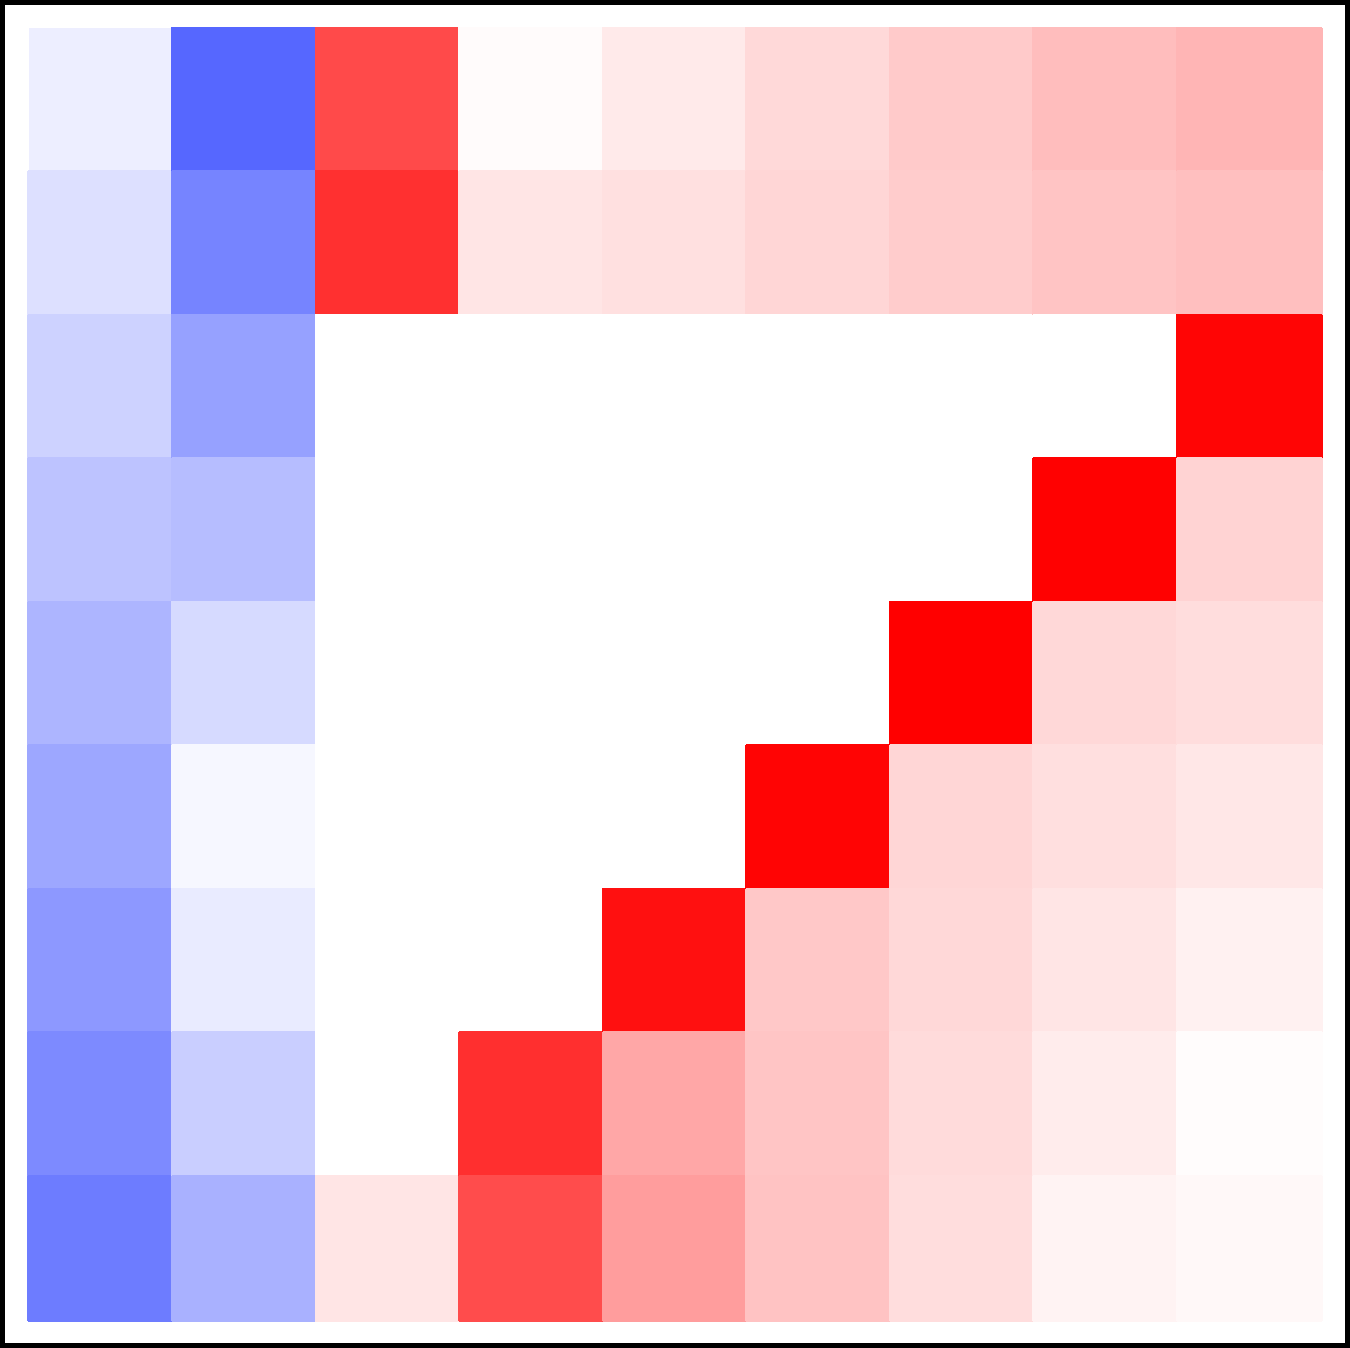
\includegraphics[ width = 6.5cm ]{\pathgraphics "bevington plus"/svd/"bevington poles"/U}  &
		  
\includegraphics[ width = 1.5cm ]{\pathgraphics "bevington plus"/svd/"bevington poles"/S}  &
		  \raisebox{3.3275\height}{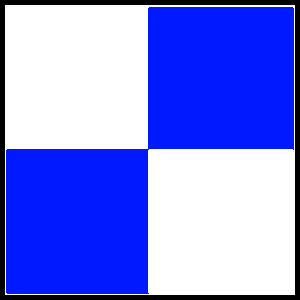
\includegraphics[ width = 1.5cm ]{\pathgraphics "bevington plus"/svd/"bevington poles"/VT}} 
		  %
		  %
		\end{tabular}
	\end{center}
	\label{tab:bevington usv block}
	\caption[Singular value decomposition for the system matrix $\A{}$.]{Singular value decomposition for the system matrix $\A{}$ in \eqref{eq:bevington axeb} showing range and null space components.}
\end{table}%

% http://cremeronline.com/LaTeX/minimaltikz.pdf
\begin{figure}[htbp] %  figure placement: here, top, bottom, or page
   \centering
    %\begin{tikzpicture}[>=stealth]
    \begin{tikzpicture}[>=latex]
      \draw [very thick] [black] [->] (0,0) -- (9.94678, 1.03034);
      \draw [very thick] [blue]  [->] (0,0) -- (9.94678, 0);
      \draw [very thick] [red]   [->] (9.94678,0) -- (9.94678, 1.03034);
      \node[] at (5.5,1) {$T$};
			\node[] at (5.5,-0.5) {\bl{$T_{\atomrng}$}};
			\node[] at (10.5,0.5) {\rd{$T_{\atomnll}$}};
    \end{tikzpicture}
   \caption{Data vector resolved into range and null space components.}
\end{figure}

  \begin{table}[htbp]  %  T A B L E
    \caption{A summary of the residual errors and their contributions to $\normt{\rd{r}}$.}
    \begin{center}
      \begin{tabular}{rrr}
        %
        $k$ & $r_{k}$ & $r_{k}^{2}$ \\\hline
        %
       1 & $-1.4$ & 1.9 \\
       2 & 6.1 & 37.6 \\
       3 & $-3.6$ & 12.7 \\
       4 & $-1.4$ & 1.8 \\
       5 & $-6.3$ & 40.3 \\
       6 & $-0.3$ & 0.1 \\
       7 & 6.5 & 41.9 \\
       8 & 9.7 & 93.7 \\
       9 & $-9.3$ & 86.7 \\
      \end{tabular}
    \end{center}
  \label{tab:bev r decomposition}
  \end{table}%

\begin{figure}[htbp] %  figure placement: here, top, bottom, or page
   \centering
    %\begin{tikzpicture}[>=stealth]
    \begin{tikzpicture}[>=latex]
      \draw [very thick] [red]   [->] (0,0) -- (10, 0);
      \draw [-] ( 0.059947, -0.1) -- (0.059947, 0.1);
      \draw [-] ( 1.24683, -0.1) -- (1.24683, 0.1);
      \draw [-] ( 1.64731, -0.1) -- (1.64731, 0.1);
      \draw [-] ( 1.7051, -0.1) -- (1.7051, 0.1);
      \draw [-] ( 2.97625, -0.1) -- (2.97625, 0.1);
      \draw [-] ( 2.97982, -0.1) -- (2.97982, 0.1);
      \draw [-] ( 4.30269, -0.1) -- (4.30269, 0.1);
      \draw [-] ( 7.26213, -0.1) -- (7.26213, 0.1);
      %\draw [-] ( 10., -0.1) -- (10., 0.1);
      %\node [] at ( 0.0299735, 0.3) {$r_{1}$};
      \node [] at ( 0.65339, 0.3) {$r_{2}$};
      \node [] at ( 1.44707, 0.3) {$r_{3}$};
      %\node [] at ( 1.67621, 0.3) {$r_{4}$};
      \node [] at ( 2.34068, 0.3) {$r_{5}$};
      %\node [] at ( 2.97804, 0.3) {$r_{6}$};
      \node [] at ( 3.64126, 0.3) {$r_{7}$};
      \node [] at ( 5.78241, 0.3) {$r_{8}$};
      \node [] at ( 8.63107, 0.3) {$r_{9}$};
    \end{tikzpicture}
   \caption{Decomposing $\normts{\rd{r} = \rd{T_{\atomnll}}}$ into residual error terms $r_{k}^2$ of table \ref{tab:bev r decomposition}.}
\end{figure}

The decomposition shown in figure \ref{fig:decomposing data vector}.
  \begin{equation*}   %  =   =   =   =   =
  \begin{array}{ccccc}
    \phantom{\frac{1}{360}}T & = & \phantom{\frac{1}{360}}\bl{T_{\atomrng}} & + & \phantom{\frac{1}{360}}\rd{T_{\atomnll}} \\
    \frac{1}{360}\mat{r}{5616 \\ 6300 \\ 13\,176 \\ 15\,768 \\ 20\,952 \\ 22\,176 \\ 23\,112 \\ 25\,344 \\ 35\,568} & = &
    \frac{1}{360}\bl{\mat{r}{5120 \\ 8507 \\ 11\,894 \\ 15\,281 \\ 18\,668 \\ 22\,055 \\ 25\,442 \\ 28\,829 \\ 32\,216}} & + &
    \frac{1}{360}\rd{\mat{r}{496 \\ -2207 \\ 1282 \\ 487 \\ 2284 \\ 121 \\ -2330 \\ -3485 \\ 3352}}
    \label{eq:archetype:data vector}
  \end{array}
  \end{equation*}

\break
\clearpage
\section{$\Q{}\R{}$ Decomposition}  %    S    S    S    S    S    S    S    S    S
Resolve the range space $\brnga{}$ into an orthonormal basis.
  \begin{equation*}   %  =   =   =   =   =
    \A{} = \Q{} \R{}
  \end{equation*}
  \begin{equation*}   %  =   =   =   =   =
    a = \R{-1}\Q{*}T
  \end{equation*}
  
\subsection{Computing the QR Decomposition}  %   SS   SS   SS   SS   SS   SS   SS   SS   SS   SS   SS   SS
$\R{}\in\real{\byy{\rho}}$
  \begin{equation*}   %  =   =   =   =   =
    \R{} = \mat{cc}{ r_{11} & r_{12} \\ 0 & r_{22} } = \mat{cc}{\nu_{1} & q_{1}^{2}a_{2} \\ 0 \nu_{2}}
  \end{equation*}
The norm of the first column vector:
  \begin{equation}
        r_{11} = \normt{a_{1}} = 3
    %\end{split}
    %\label{eqn:}
  \end{equation}
Normalized column vector
  \begin{equation}
        q_{1} = \frac{a_{1}} {r_{11}} = \frac{1}{3}\mat{c}{1\\1\\1\\1\\1\\1\\1\\1\\1}
    %\end{split}
    %\label{eqn:}
  \end{equation}
Next scale factor in row 1:
  \begin{equation}
        r_{12} = q_{1}^{*}a_{2} = 15
    %\end{split}
    %\label{eqn:}
  \end{equation}
% = =
% = =  e q u a t i o n
  \begin{equation}
        q_{2} = a_{2} - r_{12} q_{1}
    %\end{split}
    %\label{eqn:}
  \end{equation}
% = =
  \begin{equation*}   %  =   =   =   =   =
    \Q{} = 
       \mat{cc}{ \frac{1}{3} 
       \mat{c}{1 \\ 1 \\ 1 \\ 1 \\ 1 \\ 1 \\ 1 \\ 1 \\ 1} &  \frac{1}{2\sqrt{15}}
       \mat{r}{ -4 \\ -3 \\ -2 \\ -1 \\ 0 \\ 1 \\ 2 \\ 3 \\ 4 } }
  \end{equation*}
  \begin{equation*}   %  =   =   =   =   =
    \begin{array}{cccc}
      \A{} & = & \Q{} & \R{}, \\
      \mat{cc}{
         1 & 1 \\
         1 & 2 \\
         1 & 3 \\
         1 & 4 \\
         1 & 5 \\
         1 & 6 \\
         1 & 7 \\
         1 & 8 \\
         1 & 9 } & = &
       \mat{cc}{ \frac{1}{3} 
       \mat{c}{1 \\ 1 \\ 1 \\ 1 \\ 1 \\ 1 \\ 1 \\ 1 \\ 1} &  \frac{1}{2\sqrt{15}}
       \mat{r}{ -4 \\ -3 \\ -2 \\ -1 \\ 0 \\ 1 \\ 2 \\ 3 \\ 4 } } &
       \mat{cc}{ 3 & 15 \\ 0 & 2\sqrt{15} }         
    %\label{eq:}
    \end{array}
  \end{equation*}

\endinput